\documentclass[12pt]{article}

\usepackage{sbc-template}

\usepackage{float}

\usepackage{graphicx,url}

\usepackage[brazil]{babel}   
%\usepackage[latin1]{inputenc}  
\usepackage[utf8]{inputenc}  
% UTF-8 encoding is recommended by ShareLaTex

     
\sloppy

\title{Algorítmo XOR para troca de valores de variáveis}

\author{Henrique Shodi Maeta\inst{1} }


\address{Centro Universitário Senac -- (SENACSP)\\
  São Paulo -- SP -- Brazil
}

\begin{document} 

\maketitle

\section{Abstract}

\section{Introdução}

Normalmente, quando é necessário fazer a troca de valores de variáveis, é utilizado uma variável adicional como segue exemplificado na imagem abaixo:


\begin{figure}[ht]
\centering
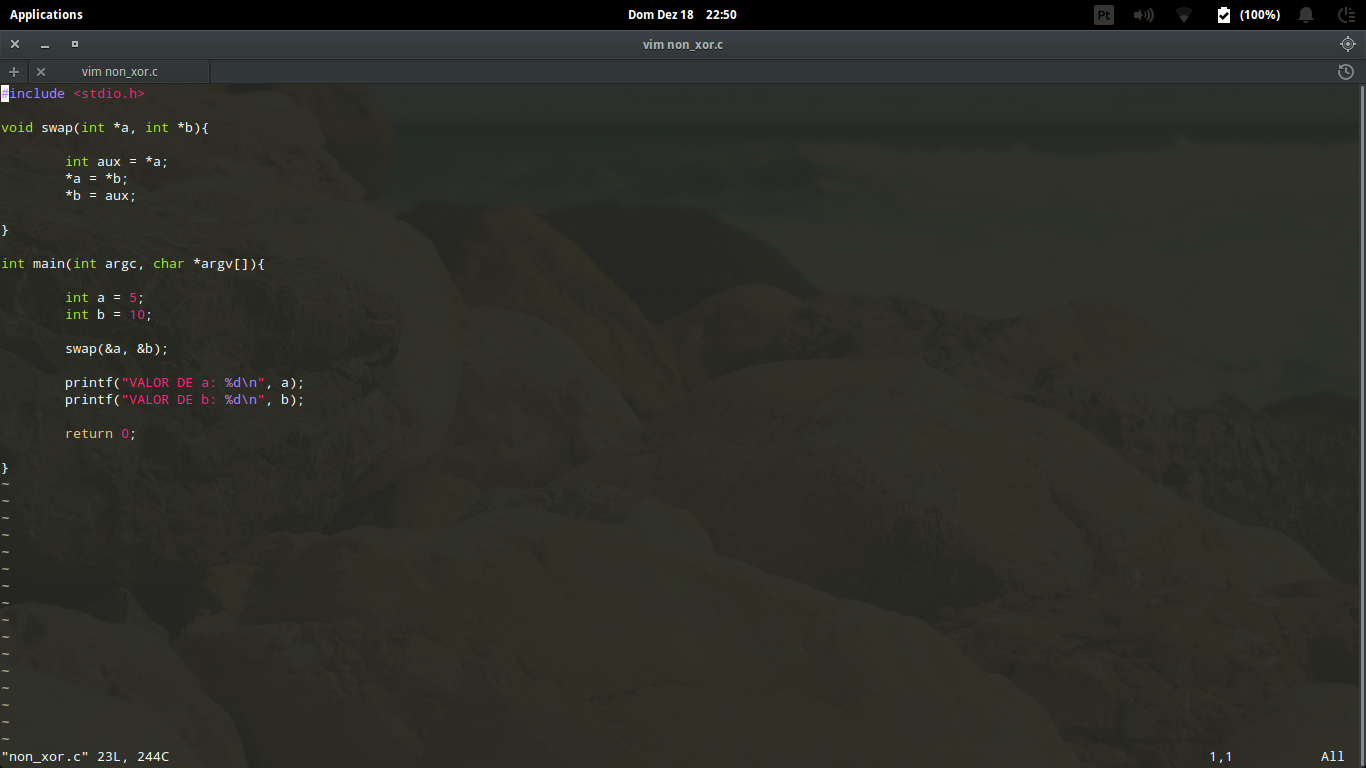
\includegraphics[width=1\textwidth]{non_xor.png}
\caption{Algorítmo para troca de valores com variável auxiliar.}
\label{fig:exampleFig1}
\end{figure}

A Figura \ref{fig:exampleFig1} mostra um algorítmo que troca o valor de duas variáveis, \textbf{\textit{a}} e \textbf{\textit{b}}, na função \textbf{\textit{swap}}. A função \textbf{\textit{swap}} recebe dois parâmetros, dois ponteiros para inteiro, pois nossa intenção é alterar o conteúdo apontado por aquele endereço de memória, e sem os ponteiros isso não seria possível. Após receber os parâmetros, iniciamos uma variável auxiliar que guardará o valor contido em \textbf{\textit{a}}, para que o mesmo possa armazenar valor encontrado no endereço apontado \textbf{\textit{b}}, fazendo com que \textbf{\textit{b}} possa copiar o valor da variável adicional para si.

Porém quando um dos principais recursos computacionais(memória) é escasso, este processo pode ser penoso e temos de ter alguns cuidados para que tal recurso não se acabe.
Um dos métodos que podemos considerar na hora de economizar memória é o algorítmo XOR para troca de valores de variáveis.
\section{Algorítmo XOR} \label{sec:firstpage}

O Algorítmo XOR(ou exclusivo) utiliza da lógica boleana para resolver este problema. Diferente do operador binário OR, onde só teremos como resposta verdadeira nos casos em que os bits analisádos forem ambos verdadeiros, ou então pelo menos um seja verdadeiro. Já o XOR só terá a resposta verdadeira caso um dos bits seja verdadeiro, como segue exemplificado na imagem abaixo:


\begin{figure}[ht]
\centering
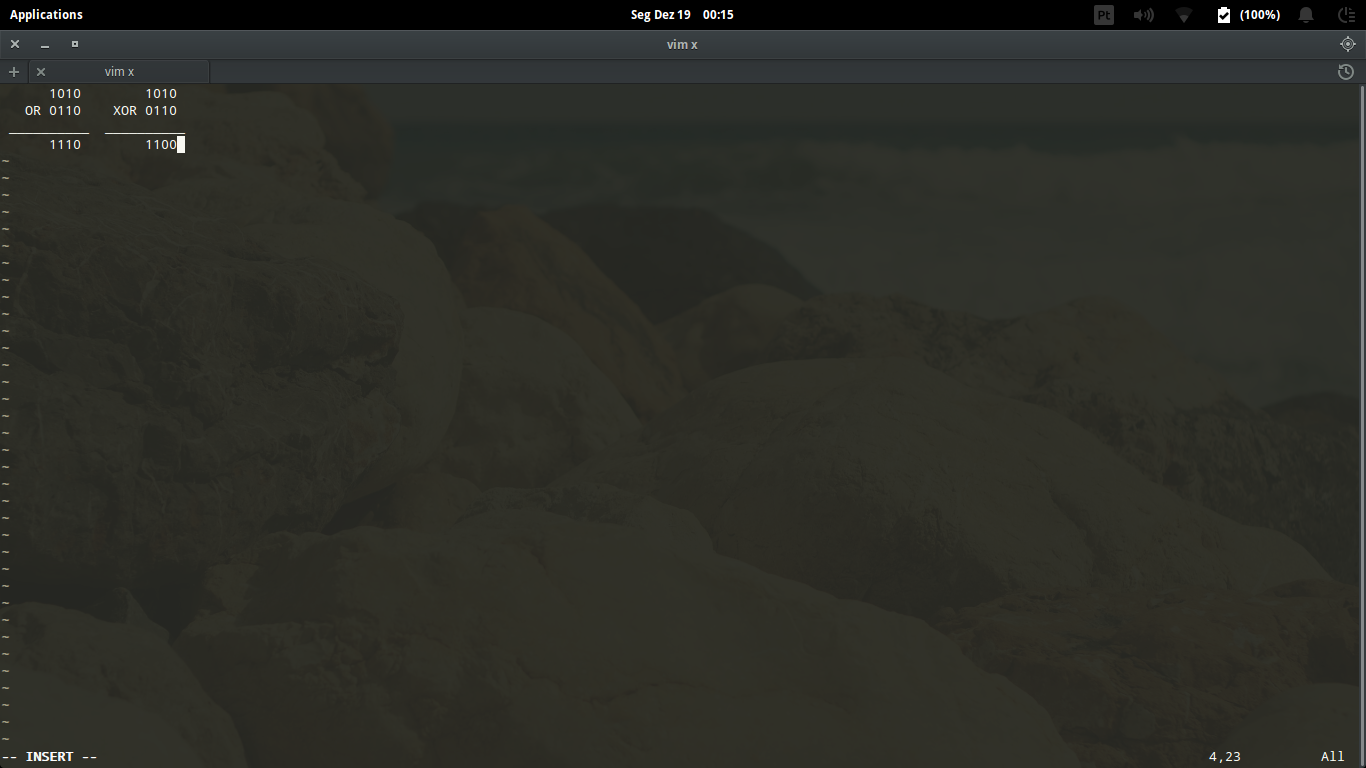
\includegraphics[width=1\textwidth]{comparacao.png}
\caption{Diferença do operador OR com XOR.}
\label{fig:exampleFig2}
\end{figure}

Com este exemplo pudemos perceber que os dois valores 10 e 6, respectivamente representados em base binária na Figura \ref{fig:exampleFig2}, geram saídas diferentes quando passam pelos operadores OR e XOR.

Com a característica do XOR podemos resolver o problema supracitado, porém sem utilizar uma varáivel auxiliar da seguinte forma:

\begin{figure}[H]
\centering
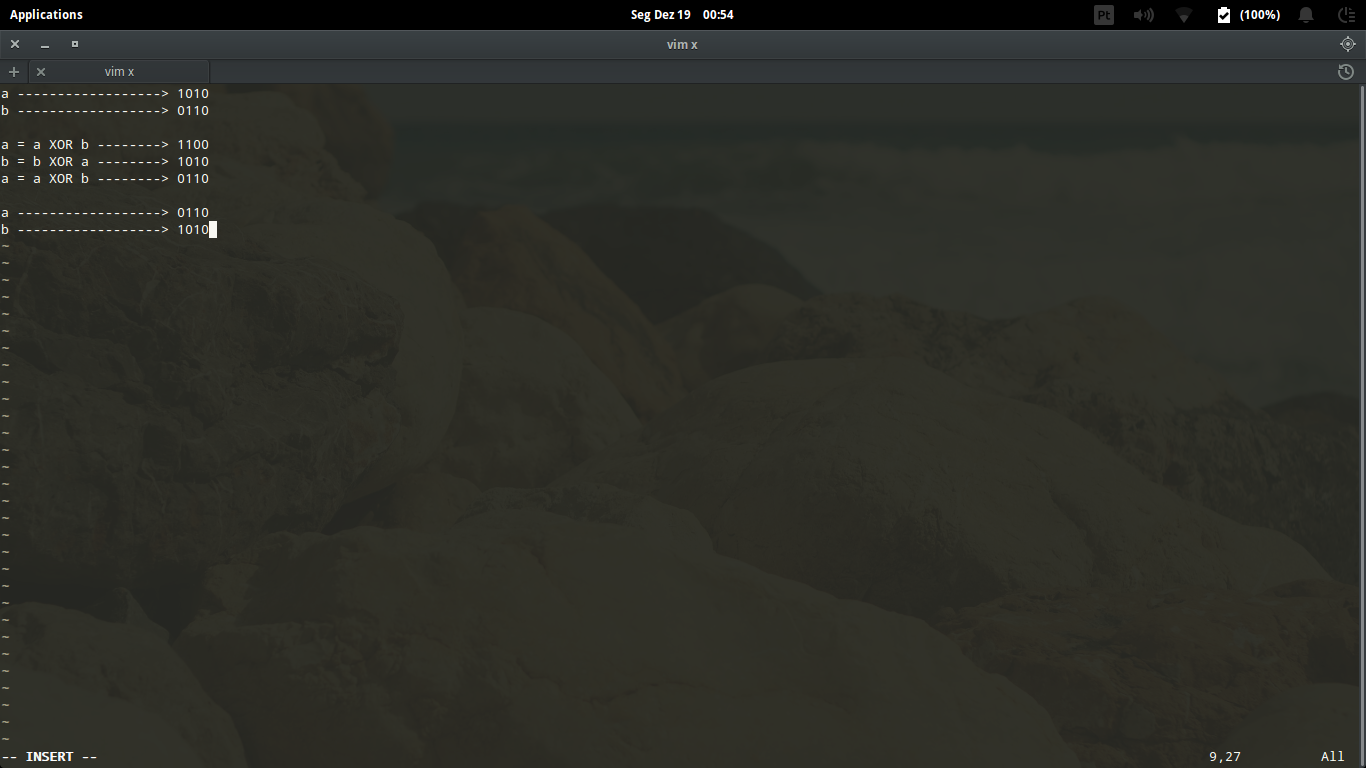
\includegraphics[width=1\textwidth]{aplicacao_xor.png}
\caption{Exemplo da aplicação do algorítmo XOR, para melhor entendimento.} 
\label{fig:exampleFig3}
\end{figure}

que por consequência faz com que nosso gasto de memória seja reduzido em 1/3 comparado com o algorítmo anterior.

\begin{figure}[H]
\centering
\includegraphics[width=1\textwidth]{xor.png}
\caption{Algorítmo XOR implementado na linguagem de programacao C.} 
\label{fig:exampleFig4}
\end{figure}


\subsection{Subsections}

The subsection titles must be in boldface, 12pt, flush left.


All images and illustrations should be in black-and-white, or gray tones,
excepting for the papers that will be electronically available (on CD-ROMs,
internet, etc.). The image resolution on paper should be about 600 dpi for
black-and-white images, and 150-300 dpi for grayscale images.  Do not include
images with excessive resolution, as they may take hours to print, without any
visible difference in the result. 


\bibliographystyle{sbc}
\bibliography{sbc-template}

\end{document}
